% Тут используется класс, установленный на сервере Papeeria. На случай, если
% текст понадобится редактировать где-то в другом месте, рядом лежит файл matmex-diploma-custom.cls
% который в момент своего создания был идентичен классу, установленному на сервере.
% Для того, чтобы им воспользоваться, замените matmex-diploma на matmex-diploma-custom
% Если вы работаете исключительно в Papeeria то мы настоятельно рекомендуем пользоваться
% классом matmex-diploma, поскольку он будет автоматически обновляться по мере внесения корректив
%

% По умолчанию используется шрифт 14 размера. Если нужен 12-й шрифт, уберите опцию [14pt]
\documentclass[12pt]{matmex-diploma-custom}
\usepackage{amsthm}
\usepackage{mathtools}
\usepackage{amssymb}
\usepackage{graphicx}
\usepackage{wrapfig}
\usepackage[caption=false]{subfig}
\usepackage{tikz}
\usepackage{pgfplots}
\pgfplotsset{compat=1.9}

\usepackage{url}
\usepackage{algpseudocode}
\usepackage{algorithm}
\usepackage{algorithmicx}
%\documentclass[14pt]{matmex-diploma-custom}

\newtheorem{mydef}{Определение}

\begin{document}
	\algnewcommand\algorithmicswitch{\textbf{switch}}
	\algnewcommand\algorithmiccase{\textbf{case}}
	\algnewcommand\algorithmicassert{\texttt{assert}}
	\algnewcommand\Assert[1]{\State \algorithmicassert(#1)}
	% New "environments"
	\algdef{SE}[SWITCH]{Switch}{EndSwitch}[1]{\algorithmicswitch\ #1\ \algorithmicdo}{\algorithmicend\ \algorithmicswitch}
	\algdef{SE}[CASE]{Case}{EndCase}[1]{\algorithmiccase\ #1}{\algorithmicend\ \algorithmiccase}
	
	\algtext*{EndSwitch}
	\algtext*{EndCase}
	\algtext*{EndWhile}% Remove "end while" text
	\algtext*{EndIf}% Remove "end if" text
	\algtext*{EndFor}% Remove "end for" text
	\algtext*{EndFunction}% Remove "end function" text
	
	% Год, город, название университета и факультета предопределены,
	% но можно и поменять.
	% Если англоязычная титульная страница не нужна, то ее можно просто удалить.
	\filltitle{ru}{
		chair              = {Программная инженерия},
		title              = {Поддержка расширенных контекстно-свободных грамматик 
			в алгоритме синтаксического анализа Generalized LL},
		type               = {bachelor},
		position           = {студента},
		group              = 471,
		author             = {Горохов Артем Владимирович},
		supervisorPosition = {к.\,ф.\,-м.\,н.,\,доц.},
		supervisor         = {Григорьев С.\,В.},
		reviewerPosition   = {СУИ НИУ ИТМО, программист},
		reviewer           = {Авдюхин Д.А.}
	}
	
	\filltitle{en}{
		chair              = {Software engineering},
		title              = {Support of extended context-free grammars in Generalized LL parsing algorithm},
		author             = {Artem Gorokhov},
		supervisorPosition = {associate professor},
		supervisor         = {Semyon Grigorev},
		reviewerPosition   = {ITMO University, programmer},
		reviewer           = {Dmitry Avduhin}
	}
	\maketitle
	%\setcounter{tocdepth}{1}
	\tableofcontents
	% У введения нет номера главы
	\section*{Введение}
	
	Общеупотребимый cпособ описания синтаксиса языков программирования ---
	расширенные контекстно-свободные грамматики. Например спецификации языков 
	$C$, $C++$, $Java$ и т.д. С одной стороны, эта форма проста для понимания людей, 
	а с другой, достаточно формальна и допускает автоматизированное создание 
	синтаксических анализаторов.
	
	Существуют различные инструменты для создания синтаксических анализаторов, которые 
	по входной грамматике позволяют создать инструментальное средство для синтаксической 
	обработки текстов, созданных на этом языке. Проблема заключается в том, что эти инструменты
	сначала преобразуют грамматику к контекстно-свободной форме, и только по ней 
	строят синтаксический анализатор.
	
	Есть работы, которые описывают синтаксический анализ с помощью расширенных
	контекстно-свободных грамматик(extended context-free grammar (ECFG)).
	Hо нет инструментов, основанных на данных работах. Кроме того, подходы, описанные
	в данных исследованиях, поддерживают лишь подклассы контекстно-свободных языков.
	
	Алгоритмы обобщённого синтаксического анализа, например Generalized LL~\cite{scott2010gll}, 
	способны использовать контекстно-свободные грамматики описывающие произвольные 
	контекстно-свободные языки. Но они так же не работают с грамматиками в форме EBNF 
	без предварительного преобразования к контекстно-свободной форме.
	
	В биоинформатике стоит задача поиска генов и иных последовательностей в геномах. 
	Эти последовательности имеют некоторые общие свойства, которые можно описать 
	контекстно-свободной грамматикой. Есть инструменты типа infernal~\cite{Infernal}, которые 
	используют синтаксический анализ для поиска структур в геномах. Но не всегда 
	генетический материал образует обычную последовательность. Метагеномные сборки - 
	результат считывания генов нескольких организмов, представленный в виде графа, пути 
	в котором задают гены этих организмов. И нет инструментов способных работать с 
	метагеномными сборками. Было бы здорово применить полученный GLL алгоритм для
	синтаксического анализа метагеномных сборок.
	
	На нашей кафедре, в рамках исследовательского проекта YaccConstructor~\cite{YaccConstructor},
	разрабатывается подход поиска структур заданных с помощью контекстно-свободной
	грамматики в метагеномных сборках, основанный на алгоритме Generalized LL.
	Предполагается, что синтаксический анализ по ECFG без преобразований даст ощутимый
	прирост производительности существующего подхода.
	
	\section{Постановка задачи}
	
	Целью данной работы является разработка модификации алгоритма GLL работающей с 
	грамматиками в расширенной форме Бэкуса-Наура и проверка того, как полученный 
	алгоритм влияет на производительность поиска структур заданных с помощью 
	контекстно-свободной грамматики в метагеномных сборках. Для её достижения были 
	поставлены следующие задачи.
	
	\begin{itemize}  
		\item Выбрать или разработать подходящее представление ECFG.
		\item Спроектировать структуру данных для представления леса разбора по ECFG.
		\item Разработать алгоритм на основе Generalized LL, строящий лес разбора по ECFG.
		\item Реализовать алгоритм в рамках проекта YaccConstructor.
		\item Провести эксперименты и сравнение.
	\end{itemize}
	
	\section{Обзор}
	
	\subsection{Расширенные контекстно-свободные грамматики}
	Статический анализ программ oбычно выполняется над структурным представлением кода. 
	И парсинг - это классический способ получить такое представление. Генераторы парсеров
	часто используются для автоматизации создания парсера: эти инструменты получают 
	парсер по грамматике.
	
	Расширенная форма Бэкуса-Наура~\cite{EBNFISO} является метасинтаксисом для представления 
	контекстно-свободных грамматик. В дополнение к конструкциям используемым в форме
	Бэкуса-Наура, в ней используется следующие конструкции: альтернатива |,
	необязательные символы [\dots], повторение {\dots} и группировка (\dots).
	
	Эта форма широко используется для спецификации грамматики в технической документации
	ввиду того, что выразительная сила ECFG делает спецификацию синтаксиса более компактной
	и удобочитаемой. Поскольку документация является одним из основных источников информации
	о языке для разработчиков синтаксических анализаторов, было бы полезно иметь генератор
	анализаторов, который поддерживает грамматики в EBNF. Заметим, что EBNF является 
	лишь стандартизированной формой для \textit{расширенных контекстно-свободных грамматик}
	~\cite{ECFG}, которые могут быть определены следующим образом:
	
	\begin{mydef}
		Расширенная контекстно-свободная грамматика (ECFG)~\cite{ECFG} - это кортеж $(N, \Sigma, P, S)$,
		где N и $\Sigma$ конечные множества нетерминалов и терминалов cоответственно, 
		$S\in N$ является стартовым символом, а P (продукция) является отображением из N в
		регулярное выражение над алфавитом $N \cup \Sigma$.
		
	\end{mydef}
	ECFG широко используется в качестве входного формата для генераторов парсеров, 
	но классические алгоритмы синтаксического анализа часто требуют CFG, и, 
	как результат, генераторы анализаторов требуют преобразования в CFG. 
	Возможно преобразование ECFG в CFG \cite{ELL}, но это преобразование приводит к увеличению
	размера грамматики и изменению её структуры: при трансформации добавляются новые
	нетерминалы. В результате синтаксический анализатор строит дерево вывода относительно
	преобразованной грамматики, и разработчику языка сложнее отлаживать грамматику 
	и использовать результат синтаксического анализа.
	
	Существует широкий спектр методов анализа и алгоритмов~\cite{AttributedELL,ELRR,
		ECFGparsing,ELLParser,ELL,ECFG,ELALR,ELRParsing}, которые способны обрабатывать 
	грамматику в ECFG. Детальный обзор результатов и задач в области обработки ECFG 
	представлены в статье ``Towards a Taxonomy for ECFG and RRPG Parsing''~\cite{ECFG}.
	Заметим только, что большинство алгоритмов основаны на классических методах
	LL~\cite{ELLParser,AttributedELL,PredictiveECFG} и LR~\cite{ELRParsing,ELALR,ELRR},
	но они работают только с ограниченными подклассами ECFG. Таким образом, нет решения 
	для обработки произвольных (в том числе неоднозначных) ECFG.
	
	Алгоритмы синтаксического анализа на основе LL более интуитивны, чем основанные на LR, и могут
	обеспечить лучшую диагностику ошибок. В настоящее время LL(1) представляется
	наиболее практичным алгоритмом. К сожалению, некоторые языки не являются LL(k) (для любого k),
	и леворекурсивные грамматики являются проблемой для инструментов на основе LL. 
	Другим ограничением для LL анализаторов являются неоднозначности в грамматике, 
	которые, вместе с предыдущими недостатками, усложняют создание синтаксических 
	анализаторов. Алгоритм Generalized LL, предложенный в~\cite{scott2010gll}, решает 
	все эти проблемы: он обрабатывает произвольные CFG, в том числе неоднозначные и
	леворекурсивные.
	В худшем случае временная и пространственная сложность GLL зависит кубически от 
	размера входа. А для LL(1) грамматик, он демонстрирует линейную временную и
	пространственную сложность.
	
	\subsection{Структурированный в виде графа стек}
	todo
	\subsection{Сжатое представление леса разбора}
	todo
	\subsection{Алгоритм Generalized LL}
	
	Цель обобщенных алгоритмов синтаксического анализа - обеспечить создание синтаксических
	анализаторов по произвольным контекстно-свободным грамматикам.
	Алгоритм Generalized LL~(GLL)~\cite{scott2010gll} включает в себя свойства классических LL алгоритмов:
	он более интуитивен и обеспечивает более хорошую диагностику ошибок, 
	чем обобщенные LR алгоритмы. Кроме того, опыт показывает, что решения на основе
	GLR более сложны, чем основанные на GLL, что согласуется с наблюдением в [11], что
	синтаксические анализаторы ECFG на основе LR очень сложны. Таким образом, в качестве
	основы для решения был выбран GLL алгоритм. 
	
	Идея алгоритма GLL основана на обработке так называемых дескрипторов, которые 
	могут однозначно определить состояние процесса синтаксического анализа. Дескриптор
	представляет собой четырехэлементный кортеж (L, i, T, S), где:
	\begin{itemize}
		\item $L$ указатель на позицию в грамматике вида~$(S \to \alpha \cdot \beta)$;
		\item $i$ --- позиция во входе;
		\item $T$ --- корень построенного леса разбора;
		\item $S$ --- текущий узел стека~(GSS)~\cite{afroozeh2015faster}.
	\end{itemize}
	
	GLL двигается одновременно по входу и грамматике, создавая множество дескрипторов
	в случае неоднозначности и использует очередь для управления обработкой дескрипторов.
	В начальном состоянии есть только один дескриптор, который состоит из начальной 
	позиции в грамматике~$(S \to \cdot \beta)$, во входе (i = 0), фиктивного узла дерева (\$)
	и дня стека. На каждом шаге алгоритм извлекает дескриптор из очереди и действует
	в зависимости от грамматики и входа. Если есть неоднозначность, то алгоритм помещает
	в очередь дескрипторы для всех возможных случаев, чтобы обработать их позже. 
	Для достижения кубической временной сложности важно помещать в очередь только дескрипторы,
	которые не создавались ранее. Для того чтобы решить добавлять дескриптор или нет
	используется глобальное хранилище всех созданных дескрипторов.
	Существует подход на основе таблиц~\cite{ragozina} для реализации GLL, который генерирует
	только таблицы для данной грамматики вместо полного кода синтаксического анализатора.
	Эта идея похожа на алгоритм в оригинальной статье и использует те же техники
	построения леса разбора и обработки стека. Псевдокод, иллюстрирующий этот подход, 
	можно найти в приложении~\ref{GLLCode}. Обратите внимание, что в эту работу не включена
	проверка для множеств first/follow.
	
	\subsection{Проект YaccConstructor}
	
	\subsection{Анализ метагеномных сборок}
	
	
	Метагеномная сборка это граф
	Анастасия Рагозина в своей магистерской предложила подход к анализу метагеномных
	сборок с помощью алгоритма GLL. Позже этот подход был модернизирован в рамках проекта.
	
	
	\section{Представление ECFG}
	
	Чтобы облегчить задание грамматики в форме ECFG для синтаксического анализатора
	будем использовать рекурсивный автомат (Recursive Automaton (RA)~\cite{tellier2006learning}
	для представления ECFG. Будем использовать следующее определение RA.
	\begin{mydef}
		Рекурсивный автомат $R$ это кортеж $(\Sigma, Q, S, F, \delta)$, где $\Sigma$
		--- конечное множество терминалов, $Q$ - конечное множество состояний, $S \in Q$ 
		--- начальное состояние, $F \subseteq Q$ --- множество конечных состояний,
		$\delta : Q \times (\Sigma \cup Q) \to Q$ --- функция перехода.
	\end{mydef}
	В рамках этой работы единственное различие между рекурсивным автоматом и общеизвестным
	конечным автоматом (FSA) состоит в том, что переходы в RA обозначаются либо терминалом ($\Sigma$),
	либо состоянием автомата ($Q$). Далее в этой работе будем называть переходы по элементам из
	$Q$ \textit{нетерминальными-переходами}, а по терминалам --- \textit{терминальными переходами}.
	
	Заметим, что позиции грамматики эквивалентны состояниям автомата, которые 
	строятся из правых частей продукций. Правые части продукций ECFG являются регулярными
	выражениями над объединенным алфавитом терминалов и нетерминалов. Итак, наша цель ---
	построить RA с минимальным числом состояний для заданной ECFG, что можно сделать следующими шагами.
	\begin{itemize}
		\item Построить конечный автомат, используя метод Томпсона для каждой правой
		части продукций.~\cite{Thompson:1968:PTR:363347.363387}.
		\item Создать карту из каждого нетерминала в соответствующее начальное состояние автомата.
		Эта карта должна оставаться консистентной на протяжение всех следующих шагов.
		\item Преобразовать автоматы из предыдущего шага в детерминированные без 
		$\varepsilon$-переходов используя алгоритм, описанный в~\cite{aho1974design}.
		\item Минимизировать детерминированные автомат, используя, например, алгоритм
		Джона Хопкрофта~\cite{hopcroft1971n}.
		\item Заменить нетерминальные переходы переходами по, стартовым состояниям автоматов,
		соответствующим данным нетерминалам, используя карту $M$. Результат 
		этого шага --- искомый рекурсивный автомат. Также используем карту $M$
		для определения функции $\Delta : Q \to N$ где $N$ --- имя нетерминала.
	\end{itemize}
	Пример преобразования ECFG в RA представлен на рис.~\ref{fig:fig1}, где состояние
	0 --- начальное состояние результирующего RA.
	\begin{figure}
		\centering
		\subfloat[Грамматика $G_1$]{
			$
			\begin{array}[b]{rl}
			S ::= a^{+} S\ b? \ | \ c \ \ \ 
			\end{array}
			$
			\label{fig:grammarG0}
		}
		~
		\subfloat[Конечный автомат для $G_1$]{
			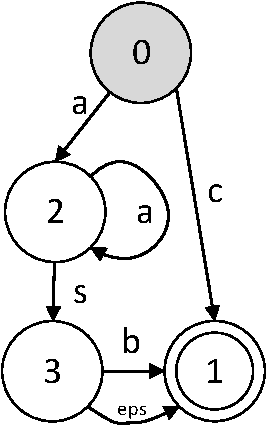
\includegraphics[scale=.6]{pictures/G0initialAutomaton.pdf}
			\label{fig:initialAutomatonsForG0}
		}
		~
		\subfloat[Рекурсивный автомат $R_1$ для $G_1$]{
			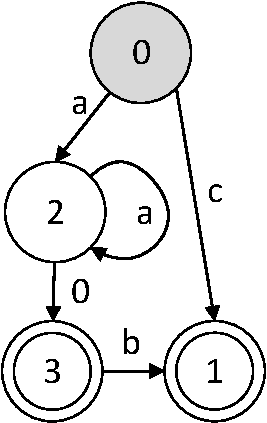
\includegraphics[scale=.6]{pictures/G0minimizedAutomaton.pdf}
			\label{fig:RAForG0}
		}
		\caption{Преобразование грамматики в рекурсивный автомат}
		\label{fig:fig1}
	\end{figure}
	
	\section{Лес разбора по ECFG}
	Результатом процесса синтаксического анализа является структурное представление 
	ввода --- дерево вывода или лес разбора в случае нескольких выводов.
	Для начала, определим дерево вывода для рекурсивного автомата: 
	это дерево, корень которого помечен начальным состоянием, листовые узлы помечены
	терминалом или $\varepsilon$, а внутренние узлы помечены нетерминалами N и их
	дети образуют последовательность меток в пути в автомате, который начинается в 
	состоянии $q_i$, где $ \Delta(q_i) = N $.
	
	\begin{mydef}
		
		Дерево вывода последовательности $\alpha$ для рекурсивного автомата $R=(\Sigma, Q, S, F, \delta)$ это дерево со следующими свойствами:
		
		\begin{itemize}
			\item Корень помечен $\Delta(S)$;
			\item Листья ---теминалы $a\in (\Sigma \cup \varepsilon)$;
			\item Остальные узлы --- нетерминалы $A\in \Delta(Q)$;
			\item У узла с меткой $N_i = \Delta(q_i)$ есть:
			\begin{itemize}
				\item 
				дети $l_0 \dots l_n (l_i \in \Sigma \cup \Delta(Q))$ тогда и только тогда,
				когда существует путь $p$ в $R$, $p = q_i \xrightarrow[]{l_0} q_{i+1} \xrightarrow[]{l_1} \dots \xrightarrow{l_n} q_m$, где
				$q_m \in F$, $l_i = 
				\left\{
				\begin{matrix}
				k_i, \text{ if }  k_i \in \Sigma,\\
				\Delta(k_i), \text{ if } k_i \in Q,
				\end{matrix}
				\right.
				$
				\item только один ребенок помеченный $\varepsilon$ тогда и только тогда,
				когда $ q_i \in F $
			\end{itemize}
		\end{itemize}
	\end{mydef}
	Для произвольных грамматик RA может быть неоднозначным с точки зрения допустимых путей,
	и, как результат, можно получить несколько деревьев разбора для одной входной строки.
	Shared Packed Parse Forest (SPPF)~\cite{SPPF} может использоваться как компактное
	представление всех возможных деревьев разбора. Будем использовать бинаризованную версию SPPF,
	предложенную в~\cite{brnglr}, для уменьшения потребления памяти и достижения кубической
	наихудшей временной и пространственной сложности. Бинаризованный SPPF может использоваться
	в GLL~\cite{scott2013gll} и содержит следующие типы узлов (здесь i и j назовём правым и
	левым extent, если i и j - начало и конец выведенной подстроки во входной строке):
	
	\begin{itemize}
		\item Упакованные узлы вида $(S, k)$, где $S$ состояние автомата, k --- начало выведенной
		подстроки правого ребёнка. У упакованных узлов обязательно есть правый ребёнок ---
		символьный узел, и опциональный левый --- символьный или промежуточный узел.
		\item Символьный узел помечен $(X, i, j)$ где $X \in \Sigma \cup \Delta(Q) \cup \{\varepsilon\}$.
		Терминальные символьные узлы ($X \in \Sigma \cup \{\varepsilon\}$) --- листья. 
		Нетерминвльные символьные узлы ($X \in \Delta(Q)$) могут иметь несколько упаковынных детей. 
		\item Промежуточные узлы помечены $ (S, i, j) $, где $S$ состояние в автомате, могут иметь несколько упаковынных детей.
	\end{itemize}
	
	Опишем модификации исходных функций построения SPPF.
	Функция \textbf{getNodeT$ (x, i) $}, которая создает терминальные узлы, 
	повторно используется без каких-либо модификаций из базового алгоритма.
	Чтобы обрабатывать недетерминизм в состояниях, определим функцию 
	\textbf{getNodes}, которая проверяет, является ли следующее состояние RA финальным
	и в этом случае строит нетерминальный узел в дополнение к промежуточному.
	Она использует изменённую функцию \textbf{getNodeP}: вместо позиции в грамматики он 
	принимает в качестве входных данных отдельно состояние RA и символ для нового узла SPPF:
	текущий нетерминал или следующее состояние RA.
	
	\begin{algorithmic}
\Function{getNodes}{$S, A, w, z$}
    \If{($S$ is final state)}
        \State $x \gets \textbf{getNodeP}(S, A, w, z)$
    \Else
        \State $x \gets \$ $
    \EndIf
    %\Statex
    %\If{$S.outedges = \varnothing$}
    %    \State $y \gets \$$
    %\Else
        \If{$(w = \$) \&$ not ($z$ is nonterminal node and it's extents are equal)}
            \State $y \gets z$
        \Else
            \State $y \gets \textbf{getNodeP}(S, S, w, z)$
        \EndIf
    %\EndIf
    
    \State \Return{$(y,x)$}
\EndFunction   
\end{algorithmic}
	\begin{algorithmic}
\Function{getNodeP}{$S, L, w, z$}
    \State $(\underline{\hspace{0.25cm}}, k, i) \gets z$
    
    \If{($w \neq \$$)}
        \State $(\underline{\hspace{0.25cm}}, j, k) \gets w$
    
        \State $y \gets$ find or create SPPF node labelled $(L, j, i)$  
    
        \If{($\nexists$ child of $y$ labelled $(S, k)$)}
            \State $y\prime \gets \textbf{new}$ $packedNode(S, k)$
            \State $y\prime.addLeftChild(w)$
            \State $y\prime.addRightChild(z)$
            \State $y.addChild(y\prime)$
        \EndIf
    
    \Else
        \State $y \gets$ find or create SPPF node labelled $(L, k, i)$ 
        \If{($\nexists$ child of $y$ labelled $(S, k)$)}
            \State $y\prime \gets \textbf{new}$ $packedNode(S, k)$
            \State $y\prime.addRightChild(z)$
            \State $y.addChild(y\prime)$
        \EndIf
    \EndIf
    \State \Return{$y$}
\EndFunction
\end{algorithmic}
	
	Рассмотрим пример SPPF для ECFG $ G_1 $~(рис.~\ref{fig:grammarG0}).
	Эта грамматика содержит конструкции (условное вхождение(?) и повторение(+)),
	которые должны быть преобразованы с использованием дополнительных нетерминалов 
	для создания обычного GLL-парсера.
	Предложенный генератор строит рекурсивный автомат $ R_1 $ ~(рис.~\ref{fig:RAForG0})
	и парсер для него. Возможные деревья ввода последовательности $ aacb $ показаны 
	на рис.~\ref{fig:treesForG0}. SPPF, созданный парсером~(рис.~\ref{fig:SPPFForG0}),
	содержит в себе все три дерева.
	
	\begin{figure}[ht]   
		\centering
		\subfloat[Возможные деревья вывода]{
			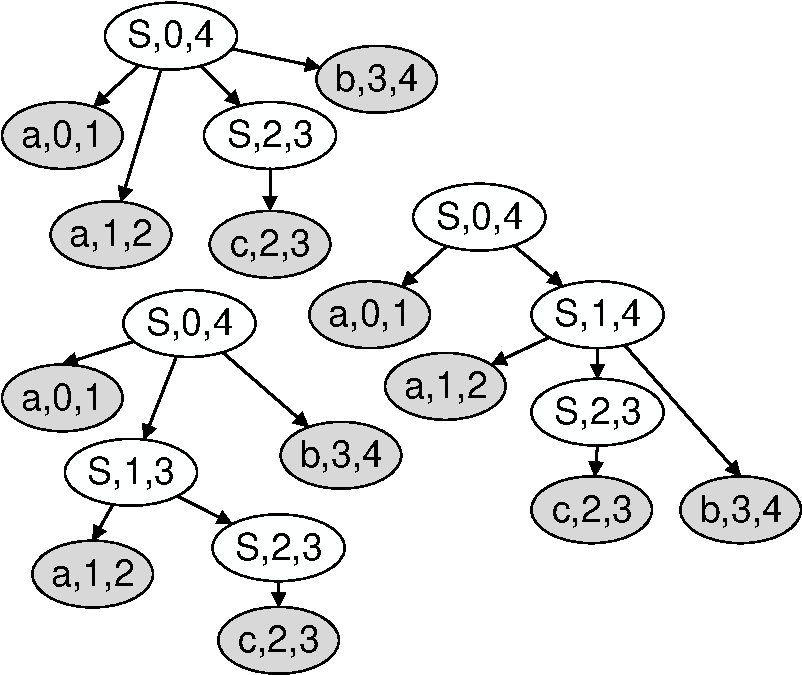
\includegraphics[scale=.5]{pictures/G0trees.pdf}
			\label{fig:treesForG0}
		}
		~
		\subfloat[SPPF]{
			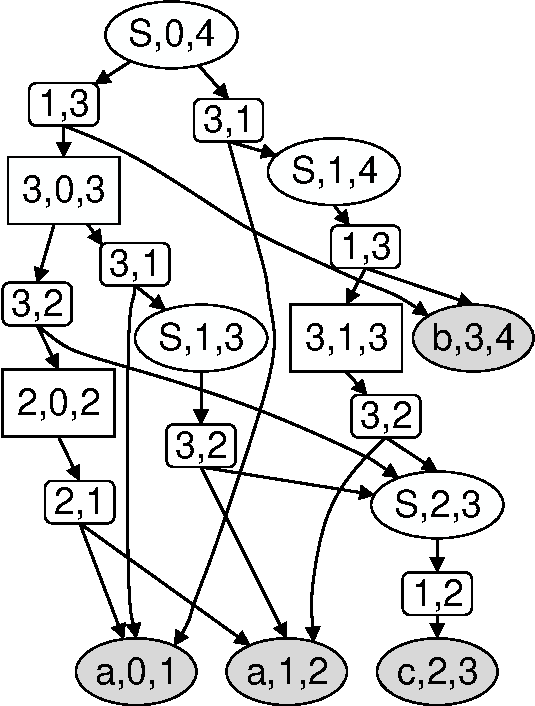
\includegraphics[scale=.5]{pictures/G0SPPFwithPackedNodes.pdf}
			\label{fig:SPPFForG0}
		}
		\caption{Пример для входа $ aacb $ и автомата $R_1$}
		\label{fig:fig2}
	\end{figure}
	
	\section{Алгоритм построения леса разбора по ECFG}
	В этом разделе мы описываем изменения в управляющих функциях базового алгоритма 
	Generalised LL, необходимые для обработки ECFG. Основной цикл аналогичен базовому
	GLL: на каждом шаге основная функция \textbf{parse} извлекает из очереди дескриптор
	$R$, подлежащий обработке. Пусть текущий дескриптор -- кортеж ($C_S, C_U, i, C_N$),
	где $C_S$ --- состояние RA, $C_U$ --- узел GSS, i --- позицию во входной строке 
	$\omega$, $C_N$ --- узел SPPF. В ходе обработки дескриптора могут возникнуть следующие
	не исключающие друг друга ситуации.
	\begin{itemize} 
		\item \textbf{$C_S$ --- финальное состояние.} Это возможно только если $C_S$
		--- стартовое состоение текущего нетерминала. Следует построить нетерминальный
		узел с ребёнком $(\varepsilon, i, i)$ и вызвать функцию \textbf{pop}, так как
		разбор нетерминала окончен.
		
		\item \textbf{Существует терминальный переход $C_S \xrightarrow[]{\omega.[i]} q$.}
		Во-первых, построить терминальный узел $ t = (\omega.[i], i, i+1) $, далее 
		вызвать функцию \textbf{getNodes} чтобы построить родителя для $ C_N $ и $ t $. 
		Функция \textbf{getNodes} возвращает кортеж $ (y, N) $, где $N$ --- опциональный
		нетерминальный узел. Создать дескриптор $ (q, C_U, i+1, y) $ и поместить в 
		очередь вне зависимости от того был ли он создан до этого. Если $ N \neq \$$,
		вызвать функцию \textbf{pop} для этого узла, состояния $ q $ и позиции во
		входе $ i + 1 $.
		
		\item\textbf{ Есть нетерминальные переходы из $C_S$.}
		Это значит что следует начать разбор нового нетерминала, поэтому должен быть
		создан новый узел GSS, если такового ещё нет. Для этого нужно вызвать функцию
		\textbf{create} для каждого такого перехода. Она осуществляет необходимые
		операции с GSS и проверяет наличие узла GSS для текущих нетерминала и 
		позиции во входе.
	\end{itemize}
	
	Псевдокод для необходимых функций представлен ниже:
	
	Функция \textbf{add} помещает в очередь дескриптор, если он не был создан до этого; эта функция не изменилась.
	\begin{algorithmic}    
\Function{create}{$S_{call}, S_{next}, u, i, w$}
    \State $A \gets \Delta(S_{call})$
    \If{($\exists$ GSS node labeled $(A, i)$)}  
    
        \State $v \gets$ GSS node labeled $(A, i)$
        \If{(there is no GSS edge from $v$ to $u$ labeled ($S_{next},w$))}
            \State add GSS edge from $v$ to $u$ labeled ($S_{next},w$)
            \For{($(v, z) \in \mathcal{P} $)}
                \State $(y,N) \gets$ \textbf{getNodes}($S_{next}, u.nonterm, w, z$)
                
                \State $(\_, \_, h) \gets y$
                \State \textbf{add}($S_{next} , u, h, y$)
                
                \If{$N \neq \$$}
                    \State $(\_, \_, h) \gets N$
                    \State \textbf{pop}$(u,h,N)$ 
                \EndIf
            \EndFor
        \EndIf
    \Else
        \State $v \gets$ \textbf{new} GSS node labeled $(A, i)$
        \State create GSS edge from $v$ to $u$ labeled ($S_{next}, w$)
        \State \textbf{add}($S_{call}, v, i, \$ $)
    \EndIf
    \Return{$v$}
\EndFunction
\end{algorithmic}  
	
	\begin{algorithmic}   
\Function{pop}{$u,i,z$}
    \If{($(u,z) \notin \mathcal{P}$)}  
        \State $\mathcal{P}.add(u,z)$
        \ForAll{GSS edges $(u,S,w,v)$}
            \State $(y,N) \gets$ \textbf{getNodes}($S, v.nonterm, w, z$)
            \If{$N \neq \$$}
                \ \textbf{pop}$(v,i,N)$ 
            \EndIf
            
            \If{$y \neq \$$}
                \ \textbf{add}($S,v,i,y$)
            \EndIf
        \EndFor
    \EndIf
\EndFunction
\end{algorithmic}
	
	%\textbf{Pop} function is called when we reach final state. It queues descriptors for all outgoing edges from current GSS node.
	
	\begin{algorithmic}
\Function{parse}{}
    \State $R.add(StartState, new GSSnode(StartNonterminal,0), 0, \$)$
    \While{$R \neq \varnothing $}
    \State{$(C_{S},C_{U},C_{i},C_{N}) \gets R.Get()$}
    \State{$C_{R} \gets \$$}
    
    \If{$(C_{N} = \$) \& (C_{S}$ is final state)}
    \State $eps \gets \textbf{getNodeT}(\varepsilon, C_{i})$  
    \State $(\underline{\hspace{0.25cm}}, N) \gets \textbf{getNodes}(C_{S},C_{U}.nonterm, \$, eps)$
    \State \textbf{pop}$(C_{U},C_{i},N)$ 
    \EndIf
    
    \For{\textbf{each} $transition (C_{S},label,S_{next})$}
        \Switch{$label$}  
        \Case{$Terminal(x)$ where ($x = input[i]$)}
            \State $R \gets \textbf{getNodeT}(x, C_{i})$
            
            \State $(y, N) \gets \textbf{getNodes}(S_{next},C_{U}.nonterm, C_{N}, R)$
            \If{$N \neq \$$}
                \State \textbf{pop}$(C_{U},i+1,N)$ 
            \EndIf
            
            \State $R.add(S_{next}, C_{U}, i + 1, y)$
            
        \EndCase
    
        \Case{$Nonterminal(S_{call})$}
    %\State{$slots \gets pTable[A][input[i]]$}
    %\If{$slots \neq \varnothing$}
            \State \textbf{create}($S_{call}, S_{next}, C_{U}, C_{i}, C_{N}$)
    %\EndIf
    %\ForAll{$L \in slots$}
    %    \State{\Call{add}{L,u,i,\$}} 
    %\EndFor
        \EndCase
        \EndSwitch
        
    \EndFor
    \EndWhile
\EndFunction
\end{algorithmic}
	
	\section{Реализация}
	\section{Эксперименты}
	
	\section*{Заключение}
	В рамках данной работы разработана и реализована модификация алгоритма GLL,
	работающая с расширенными контекстно-свободными грамматиками и показано, что полученный
	алгоритм повышает производительность поиска структур заданных с помощью контекстно-свободной
	грамматики в метагеномных сборках. Более детально, были получены следующие результаты:
	\begin{itemize}
		\item В качестве подходящего представления ECFG выбраны рекурсивные конечные автоматы.
		\item Спроектирована структура данных для представления леса разбора по ECFG 
		на основе сжатого леса разбора(SPPF).
		\item Разработан алгоритм на основе Generalized LL, строящий лес разбора по ECFG.
		\item Алгоритм реализован в рамках проекта YaccConstructor.
		\item Проведены эксперименты, показавшие двухкратный прирост 
		производительности на имеющихся метагеномных сборках по сравнению 
		с существуюшим решением.
		\item Результаты работы успешно представлены на международной конференции
		``Tools and Methods of Program Analysis''(Москва, 2017г.)
	\end{itemize}
	
	\setmonofont[Mapping=tex-text]{CMU Typewriter Text}
	\bibliographystyle{ugost2008ls}
	\bibliography{diploma.bib}
	\section{Dataset description}\label{section:dataset}

In our evaluation we use dataset which contains the following parts.
{\setlength{\tabcolsep}{0.4em}
	\begin{table}[h]
		\caption{RDFs properties}
		\label{tbl:propRDF}
		\rowcolors{2}{}{lightgray}
		\begin{tabular}{| l | c | c | c | c |}
			\hline
			Name                  & \#V    & \#E     & \#type &\#subClassOf \\
			\hline
			\hline
			atom-primitive				& 291		& 685		& 138	& 122	\\
			univ-bench					& 179		& 413		& 84		& 36		\\
			travel						& 131		& 397		& 90		& 30		\\
			skos							& 144		& 323		& 70		& 1		\\
			people\_pets					& 337		& 834		& 161	& 33		\\
			generations					& 129		& 351		& 78		& 0		\\
			foaf							& 256		& 815		& 174	& 10		\\
			biomed-mesure-prim   	    & 341		& 711		& 130	& 122	\\
			funding						& 778		& 1480		& 304	& 90               \\
			pizza						& 671		& 2604		& 365	& 259              \\
			wine							& 733		& 2450		& 485	& 126              \\
			core							& 1323		& 8684		& 1412	& 178              \\
			pathways						& 6238		& 37196		& 3118 	& 3117             \\
			go-hierarchy					& 45007		& 1960436	& 0		& 490109           \\
			enzyme						& 48815		& 219390		& 14989	& 8163             \\
			eclass\_514en				& 239111		& 1047454	& 72517	& 90962            \\
			go							& 272770		& 1068622	& 58483	& 90512            \\
			\hline
		\end{tabular}
	\end{table}
}

{\setlength{\tabcolsep}{0.4em}
\begin{table*}[h]
\caption{RDFs query $G_2$ (time is measured in seconds and memory is measured in megabytes)}
\label{tbl:tableRDFQ2}
\rowcolors{3}{}{lightgray}
\begin{tabular}{| l | r  r | r  r | r  r | r  r | r  r |}
    \hline

    \multirow{3}{*}{Name}   &   \multicolumn{6}{|c|}{Relational semantics index}	&	\multicolumn{4}{|c|}{Single path semantics index} \\
    \cline{2-11}
    &	\multicolumn{2}{|c|}{RG\_CPU\textsubscript{rel}}	&	\multicolumn{2}{|c|}{RG\_CUSP\textsubscript{rel}}	&	\multicolumn{2}{|c|}{RG\_SPARSE\textsubscript{rel}} &	\multicolumn{2}{|c|}{RG\_CPU\textsubscript{path}}	&	\multicolumn{2}{|c|}{RG\_SPARSE\textsubscript{path}}	 \\
    \cline{2-11}
    &   Time & Mem &  Time     & Mem & Time     & Mem  &  Time     & Mem & Time     & Mem \\
    \hline
    \hline
    atom-primitive          & 0.001 & 0.3  & 0.001 & 0.1 & 0.002 & 0.1   & 0.001 & 0.3  & 0.002 & 0.1   \\
biomedical-mesure-primitive & 0.002 & 0.1  & 0.014 & 2.0   & 0.009 & 0.1   & 0.006 & 0.1  & 0.012 & 0.1   \\
core                        & 0.001 & 0.3  & 0.006 & 0.1 & 0.004 & 0.1   & 0.003 & 0.3  & 0.005 & 0.1   \\
eclass\_514en               & 0.035 & 6.5  & 0.020 & 16.0  & 0.100   & 12.0    & 0.123 & 17.7 & 0.127 & 18.0    \\
enzyme                      & 0.006 & 3.9  & 0.006 & 0.6 & 0.010  & 0.1   & 0.012 & 5.3  & 0.008 & 0.4   \\
foaf                        & 0.001 & 0.1  & 0.004 & 0.1 & 0.002 & 0.1   & 0.001 & 0.1  & 0.003 & 0.1   \\
funding                     & 0.002 & 0.1  & 0.015 & 0.4 & 0.007 & 0.1   & 0.009 & 0.1  & 0.008 & 0.1   \\
generations                 & 0.001 & 0.1  & 0.001 & 0.1 & 0.001 & 0.1   & 0.001 & 0.1  & 0.001 & 0.1   \\
go-hierarchy                & 0.095 & 17.8 & 0.253 & 528.0 & 0.175 & 130.4 & 0.884 & 88.8 & 0.306 & 138.8 \\
go                          & 0.306 & 25.8 & 0.240 & 84.0  & 0.181 & 25.4  & 0.918 & 78.1 & 0.219 & 34.2  \\
pathways                    & 0.005 & 0.2  & 0.005 & 0.4 & 0.004 & 0.1   & 0.017 & 0.5  & 0.003 & 0.1   \\
people\_pets                & 0.001 & 0.1  & 0.007 & 0.1 & 0.004 & 0.1   & 0.001 & 0.1  & 0.005 & 0.1   \\
pizza                       & 0.002 & 0.3  & 0.012 & 0.2 & 0.008 & 0.1   & 0.010  & 0.3  & 0.009 & 0.1   \\
skos                        & 0.001 & 0.1  & 0.001 & 0.1 & 0.001 & 0.1   & 0.001 & 0.1  & 0.002 & 0.1   \\
travel                      & 0.001 & 0.1  & 0.007 & 0.1 & 0.005 & 0.1   & 0.001 & 0.1  & 0.005 & 0.1   \\
univ-bench                  & 0.001 & 0.1  & 0.007 & 0.1 & 0.005 & 0.1   & 0.001 & 0.1  & 0.005 & 0.1   \\
wine                        & 0.001 & 0.3  & 0.006 & 0.1 & 0.004 & 0.1   & 0.002 & 0.3  & 0.004 & 0.1  \\
    \hline
  \end{tabular}
\end{table*}
}

\begin{itemize}
\item The real-world data RDFs provided in CFPQ\_Data dataset\footnote{CFPQ\_Data dataset GitHub repository: \url{https://github.com/JetBrains-Research/CFPQ_Data}. Access date: 12.11.2019.} from~\cite{Mishin:2019:ECP:3327964.3328503}.
\item Geospecies (RDF which contains information about biological hierrarchy\footnote{The Geospecies RDF: \url{https://old.datahub.io/dataset/geospecies}. Access date: 12.11.2019.} and same-generation query over \textit{broaderTransitive} relation) is provided in~\cite{Kuijpers:2019:ESC:3335783.3335791} and integrated in our evaluation with CFPQ\_Data.
\item It was shown in~\cite{Mishin:2019:ECP:3327964.3328503} that matrix-based algorithm is performant enough to handle bigger RDFs than those used in the initial datasets, such as~\cite{RDF}.
So, we add several big RDFs to CFPQ\_Data and use them in our evaluation.
New RDFs: \textit{go-hierarchy, go, enzime, core, pathways} are from UniProt database\footnote{Protein sequences data base: \url{https://www.uniprot.org/}. RDFs with data are avalable here: \url{ftp://ftp.uniprot.org/pub/databases/uniprot/current_release/rdf}. Access date: 12.11.2019}, and \textit{eclass-514en} is from eClassOWL project\footnote{eClassOWL project: \url{http://www.heppnetz.de/projects/eclassowl/}. eclass-514en file is available here: \url{http://www.ebusiness-unibw.org/ontologies/eclass/5.1.4/eclass_514en.owl}. Access date: 12.11.2019.}.
\end{itemize}

The properties of the RDFs from the dataset are given in table \ref{tbl:propRDF}. 
Geospecies RDF contains 450609 vertices, 2311461 edges, and 20867 edges labeled by \textit{broaderTransitive}.
Note that while the number of edges labeled by \textit{broaderTransitive} is equal to provided in~\cite{Kuijpers:2019:ESC:3335783.3335791}, the total number of vertices and edges is bigger. It is because we naively convert each triple from RDF to edge in the graph, while J. Kuijpers et al. use special \textit{neosemantics}\footnote{Neosemantix is an RDF processing plugin for Neo4j. Web page: \url{https://neo4j.com/labs/nsmtx-rdf/}. Access date: 30.03.2020.} plugin which can, for example, handling multivalued properties accurately.  

The variants of the \textit{same-generation query}~\cite{FndDB} are used in almost all cases because it is an important example of real-world queries that are context-free but not regular.
So, variations of the same generation query are used in our evaluation.
All queries are added to the CFPQ\_Data dataset.

We use two queries over \textit{subClassOf} and \textit{type} relations.
The first query is the grammar $G_1$:
\[
 \begin{array}{lcl}
   s  \rightarrow \textit{subClassOf}^{\ -1} \ s \ \textit{subClassOf}   & \quad & s  \rightarrow \textit{type}^{\ -1} \ s \ \textit{type}     \\
   s  \rightarrow \textit{subClassOf}^{\ -1} \ \textit{subClassOf}       & \quad & s  \rightarrow  \textit{type}^{\ -1}  \ \textit{type}

 \end{array}
 \]
The second one is the grammar $G_2$: \[s \rightarrow \textit{subClassOf}^{\ -1} \ s \ \textit{subClassOf} \mid \textit{subClassOf}\]

For geospecies we use same-generation query \textit{geo} from the original paper~\cite{Kuijpers:2019:ESC:3335783.3335791}: \[s \rightarrow \textit{broaderTransitive} \ s \ \textit{broaderTransitive}^{\ -1} \]
\[s \rightarrow \textit{broaderTransitive}  \ \textit{broaderTransitive}^{\ -1} \]


\section{Evaluation Details}

Results for RDFs querying with $G_2$ grammar are presented in table~\ref{tbl:tableRDFQ2}.
We can see, that for small graphs time for both relational and single-path querying are similar for CPU and GPGPU versions, but for bigger graphs (\textit{go} and \textit{go-hierarchy}, for example) GPUPU version is more performant than CPU one.

\balance


\end{document}
